%\section[Boosting To Residuals \\~\\ 残差にブースティング]{残差にブースティング Boosting To Residuals}

\begin{frame}{Setup}
シンプルなセットアップから出発する.\\~\\

$\{ x_i, y_i \}$ はデータセットを表す.\\~\\

$N$ はトレーニングサンプルの数を指し,  $M$ は特徴量の数を指す.
\end{frame}
%

\begin{frame}{Setup}
回帰という文脈においては,

$$ y_i \approx f(x_i) \ \text{for all} \ i $$

つまり

$$\argmin_{f} \underbrace{\frac{1}{N}\sum_i  ^ N\left( y_i - f(x) \right)^2}_{\textit{Mean Squared Error (MSE)}}$$

となる$f$を探すのが目的である.

\end{frame}
%

\begin{frame}{Setup}
最終的に, $f$ は\textit{弱い}学習器の和として表現される
$$ \underbrace{f(x)}_{\textit{final model}} \!\!\!\!\! = \underbrace{f_0(x) + f_1(x) + f_2(x) + \cdots + f_{\text{max}}(x)}_{\textit{weak learners}} $$
モデルを作る段階は以下のように表せる:
\begin{align*}
    S_0(x) &= f_0(x) \\
    S_1(x) &= f_0(x) + f_1(x) \\
    S_2(x) &= f_0(x) + f_1(x) + f_2(x) \\
    &\vdots \\
    S_{k + 1} (x) &= S_{k}(x) + f_{k+1}(x)
\end{align*}
$S$は各段階でのモデルを表しており,最終段階では$S_{max}$でモデルが完成する.\\~\\

\end{frame} 
%
\begin{frame}{Optimizing}
全ての段階で目指すのは$S$による$y$(観察されたトレーニングデータ)の近似である.
$$S_{k + 1} (x) = S_{k}(x) + f_{k+1}(x) \approx y$$
この時の弱学習器$f_{k+1}$に着目して並べ替えると,
$$f_{k + 1} (x) \approx \underbrace{y - S_{k}(x)}_{\textit{Residual}}$$
つまり各段階で前段階のモデルの残差項に$x$を回帰していき,最適な$f$を得る.
\end{frame}
%
\begin{frame}
Gradient Boosting では,段階を追って調整しながらモデルの$f$を決める.

  \begin{figure}
    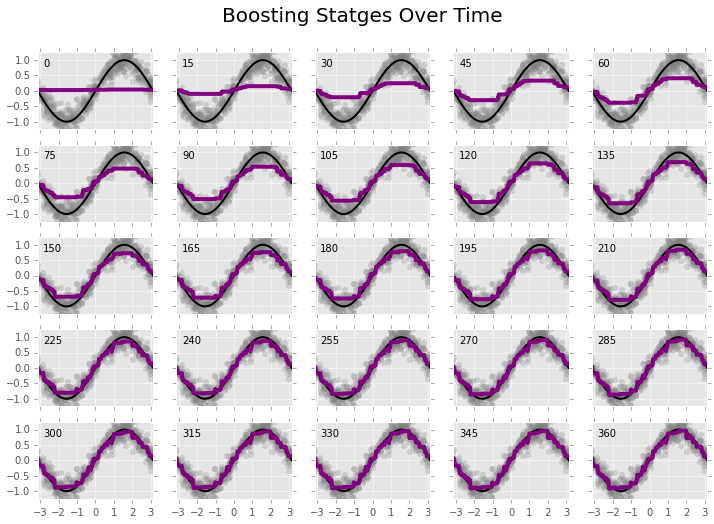
\includegraphics[scale=0.35]{boosting-over-time-multiple-plots}
    \caption{Boosting による段階的近似, borrowed from Matthew Drury}
  \end{figure}
  
\end{frame}
%

\begin{frame}{図で段階を追う}
まず$S_0(x) = f_0(x)$だが,この時MSEを最小化する値は言わずとも
$$ f_0(x) = \frac{1}{N} \sum_i y_i $$
  \begin{figure}
    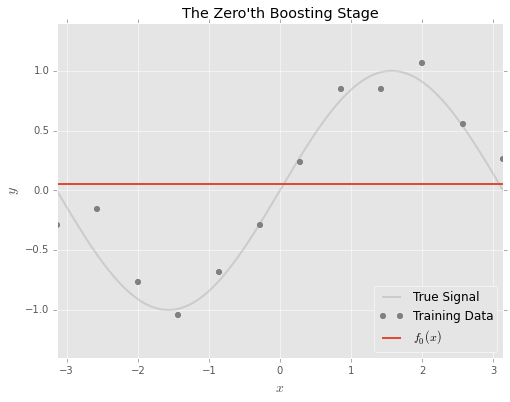
\includegraphics[scale=0.45]{zeroth-boosting-stage}
  \end{figure}
  %次段階では,$S_1(x) = f_0(x) + f_1(x)$へモデルを更新する.

\end{frame}
%

\begin{frame}
残差である$y_i - f_0(x_i)$の方向へモデルを調整していく! \\
この際,トレーニングデータが存在する点でしか残差は定義されない \\~\\
$\to$ 回帰を通じて残差にモデルをフィットする!

  \begin{figure}
   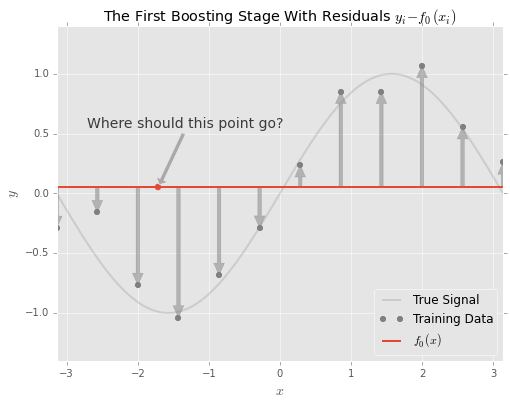
\includegraphics[scale=0.4]{first-boosting-stage-with-residuals-dillema}
  \end{figure}
  
\end{frame}
%

\begin{frame}{$f_1(x)$を計算する}
残差を新たなデータセットとして,決定木回帰により最初のTree$f_1(x)$を推定する.

  \begin{figure}
    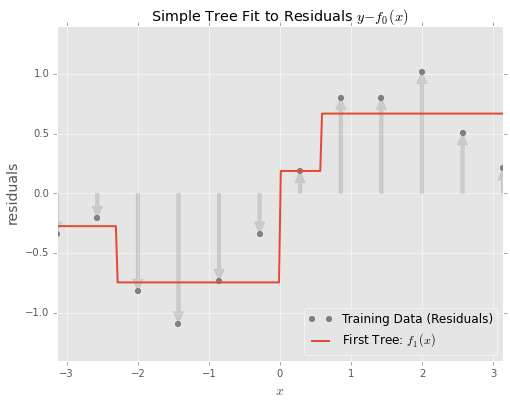
\includegraphics[scale=0.45]{first-boosting-stage-residuals-with-tree}
  \end{figure}

\end{frame}
%

\begin{frame}{モデルの更新}

$$S_1(x) = f_0(x) + f_1(x) \leftarrow \text{Model fit to residuals!}$$

  \begin{figure}
    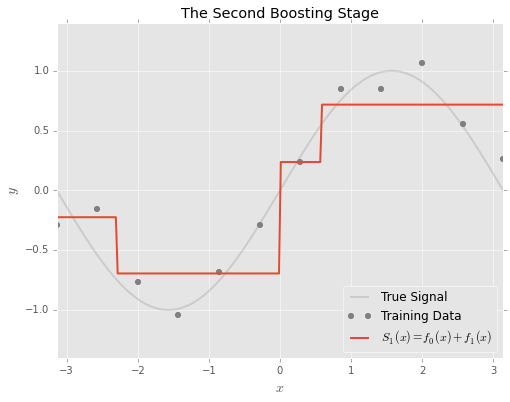
\includegraphics[scale=0.45]{second-boosting-stage}
  \end{figure}
  
\end{frame}
%

\begin{frame}{Another Step}
現時点のモデルの残差を計算...

  \begin{figure}
    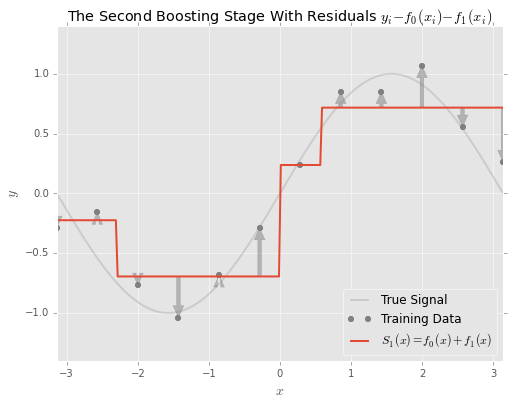
\includegraphics[scale=0.50]{second-boosting-stage-with-residuals}
  \end{figure}
  
\end{frame}
%

\begin{frame}
残差が被説明変数となるようなトレーニングデータセットを作る...

  \begin{figure}
    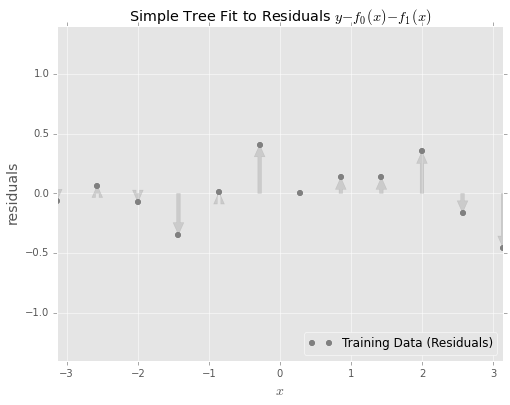
\includegraphics[scale=0.50]{second-boosting-stage-residual-training-set}
  \end{figure}
  
\end{frame}
%

\begin{frame}
モデルに追加する弱学習器を推定する

  \begin{figure}
    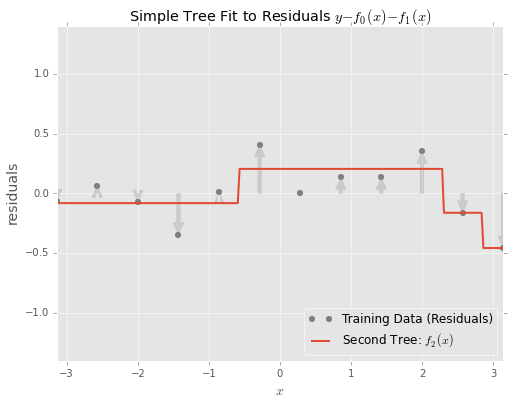
\includegraphics[scale=0.50]{second-boosting-stage-residuals-with-tree}
  \end{figure}
  
\end{frame}
%

\begin{frame}
モデルの更新!

  \begin{figure}
    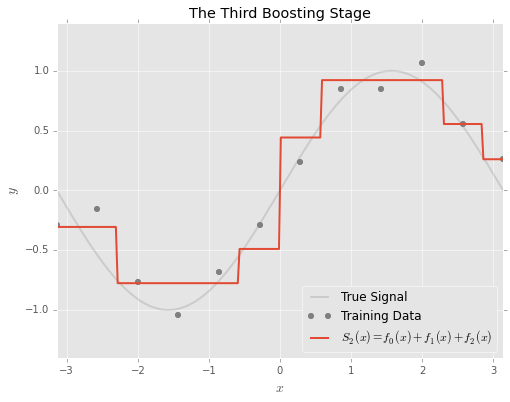
\includegraphics[scale=0.50]{third-boosting-stage}
  \end{figure}
  
\end{frame}
%

\begin{frame}{漸近的に近づける!}

  \begin{figure}
    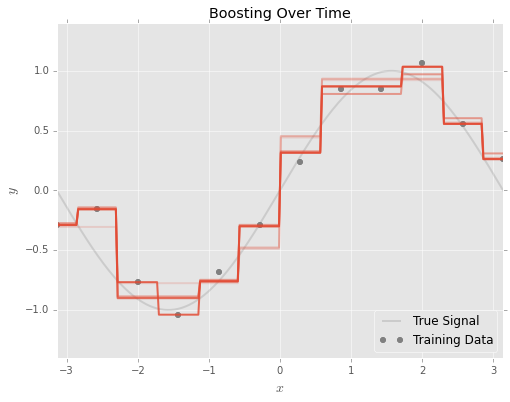
\includegraphics[scale=0.50]{simple-boosting-over-time}
  \end{figure}
  
\end{frame}
%

\begin{frame}{損失関数}
先ほどまでの例ではMSEを損失関数として使用\\~\\
それに限らず,損失関数$L\left(y, S(x)\right)$を定義できる$\downarrow$
$$S_{k + 1}(x) = S_k(x) + \argmin_{f} \sum^N_{i=1}L(y_i, S_k(x_i) + f_{k+1}(x_i))$$
しかし,毎回グローバルなミニマムを探すのは難しい...\\
$\to$ 勾配法を導入, ローカルな極小を発見
$$S_{k + 1}(x) = S_k(x) - \left[\sum^N_{i=1}\nabla_{S_k}L(y_i, S_k(x_i))\right]$$
\begin{center}
  \textbf{\textcolor{red}{Gradient Boosting!}}
\end{center}

\end{frame}
%


\begin{frame}{勾配降下法}

最急勾配法は任意の微分可能な関数$L(x)$の最適化手法 \\~\\

\textbf{Inputs:} 関数 $L$. \\~\\

\textbf{Outputs:} $L$を最小化する点$x^*$. \\~\\

\textbf{Algorithm:} $x$が$x^*$へ収束するまで$x_{i+1} = x_i - \lambda \nabla L(x_i)$を繰り返す.


\end{frame}
%

\begin{frame}{Gradient Boosting}
$$S_{k + 1}(x) = S_k(x) - \left[\sum^N_{i=1}\nabla_{S_k}L(y_i, S_k(x_i))\right]$$
\begin{center}
  \textbf{\textcolor{red}{Gradient Boosting!}}
\end{center}

\end{frame}
%


\begin{frame}{弱学習器のウェイト}
モデル更新の際,全ての弱学習器をただモデルに足していくのではなく,ウェイトを付加することで予測性能をさらに上げる.
$$S_{k+1}(x) = S_k(x) + \lambda_{k+1} f_{k+1}(x)$$
$$\left ( = S_k(x) - \lambda_{k+1} \sum^N_{i=1} \nabla_{S_k} L(y_i, S_k(x_i)) \right )$$
この時,
\begin{align*}
\lambda_{k+1} &= \argmin_{\lambda} \sum^{N}_{i = 1}L\left(y_i, S_{k+1}(x_i)\right) \\
& =\argmin_{\lambda} \sum^{N}_{i = 1}L\left(y_i, S_k(x_i) + \lambda_{k+1} f_{k+1}(x_i)\right)
\end{align*}
\end{frame}
%

\begin{frame}{ウェイトによる滑らかな近似}

  \begin{figure}
    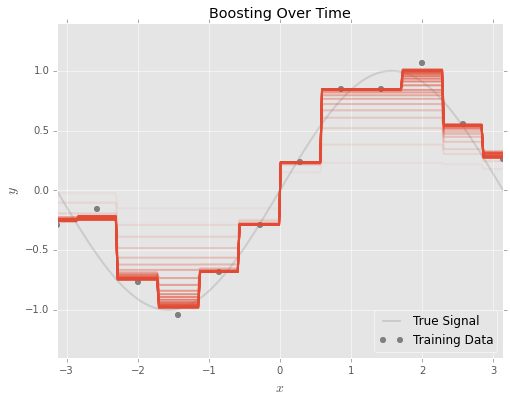
\includegraphics[scale=0.50]{simple-boosting-over-time-learning-rate}
  \end{figure}

\end{frame}
%

\begin{frame}{Gradient Tree Boosting}

GTBは使われている弱学習器が決定木の場合をいう. \\
\begin{itemize}
\item 決定木のリーフの数を$J_k$とする
\item 木はフィーチャースペースを$R_{1,k}, \dots, R_{J_k, k}$に分画する.
\end{itemize}
$$f_k(x) = \sum_{j = 1}^{J_m} \underbrace{b_jm}_{R_{jm}\text{の予測値}}\!\!\!\!\mathbbm{1}_{R_{jm}}(x)$$ % Note: in case of usual CART trees, the trees are fitted using least-squares loss, and so the coefficient {\displaystyle b_{jm}}b_{jm} for the region {\displaystyle R_{jm}}R_{jm} is equal to just the value of output variable, averaged over all training instances in {\displaystyle R_{jm}}R_{jm}.
\end{frame}
%


\begin{frame}{ちなみに...}
最小二乗法に勾配降下法を当てはめると,
\begin{align*}
x_{k+1} &= x_k - \lambda \nabla_x L(x_k, y) \\
&= x_k - \lambda \nabla_x \frac{\partial}{\partial x}\left(\frac{1}{2}(y - x_k)^2\right) \\
&= x_k + \lambda(y - x_k)
\end{align*}
つまり,最小二乗法のもとでは段階的に残差の方向に向かって動いていく.
\end{frame}
%

\begin{frame}{復習}

\textbf{Inputs:} A training data set $\{ x_i, y_i \}$, and, optionally, a learning rate $\lambda$ to replace weights.

\textbf{Returns:} A function $f$ such that $f(x_i) \approx y_i$.

\begin{itemize}
  \item Initialize $S_0(x) = f_0(x) = \frac{1}{N} \sum_i y_i$.
  \item Iterate (parameter $k$) until satisfied: \begin{itemize}
    \item Create the working data set $W_k = \{ x_i, y_i - S_{k}(x_i) \}$.
    \item Fit a regression tree to $W_k$, minimizing least squares.  Call this tree $f_k$.
    \item Set $S_{k+1}(x) = S_{k}(x) + \lambda f_{k}(x)$. 
  \end{itemize}
  \item Return $f_{\text{max}}(x) = f_0(x) + f_1(x) + f_2(X) + \cdots + f_{\text{max}}(x)$.
\end{itemize}

\end{frame}
%